\chapter{Lec 23 - Structured Probabilistic Models II}

\section{Learning about Dependencies}
We know that graphs can be used to represent in an efficient way the factorization of joint probability distributions, but how can we find the correct factorization given a specific distribution? There are two main families of approaches:
\begin{itemize}
    \item Learning Graph Structure
    \item Use Latent Variables
\end{itemize}

\subsection{Learning Graph Structure}
When the model is intended to capture dependencies between visible variables
with direct connections, it is usually infeasible to connect all variables, so the graph must be designed to connect those variables that are tightly coupled and omit edges between other variables. An entire field of machine learning called \textbf{structure learning} is devoted to this problem.\newline\newline
Most structure learning techniques are a form of greedy search in the space of all possible graphs. A structure is proposed, a model with that structure
is trained, then given a score. The score rewards high training set accuracy and penalizes model complexity. Candidate structures with a small number of edges added or removed are then proposed as the next step of the search. The search proceeds to a new structure that is expected to increase the score.

\subsection{Use Latent Variables}
In the context of deep learning, the approach most commonly used to model the dependencies between the observed variables $\textbf{v}$ is to introduce several latent or “hidden” variables $\textbf{h}$. The model can then capture dependencies between any pair of variables $v_i$ and $v_j$ indirectly, via direct dependencies between $v_i$ and $\textbf{h}$, and
direct dependencies between $\textbf{h}$ and $v_j$. Using latent variables instead of adaptive structure avoids the need to perform discrete searches and multiple rounds of training. Note that in this case we are assuming that the visible variables depend on some latent non-observable variables.\newline\newline
A fixed structure over visible and hidden variables can use direct interactions between visible and hidden units to impose indirect interactions between visible units. Using simple parameter learning techniques we can learn a model with a fixed structure that imputes the right structure on the marginal $P(\textbf{v})$. 
\begin{center}
    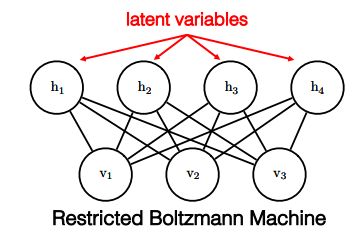
\includegraphics[]{images/RBM.png}
\end{center}
Obviously, we need to make an assumption regarding the number of latent variables we want to fix (just like the number of hidden units in a neural network). Furthermore, we usually set dense connections of latent variables to observed variables.

\section{Inference and Approximate Inference}
With \textbf{inference} we mean the task of predicting the value of some variables given other variables, or predicting the probability distribution over some variables given the value of other variables.\newline\newline
For example, in a latent variable model we might want to extract features $E[\textbf{h} | \textbf{v}]$ describing the observed variables $\textbf{v}$.\newline\newline
Unfortunately, for most interesting deep models, these inference problems are intractable, even when we use a structured graphical model to simplify them. The graph structure allows us to represent complicated, high-dimensional distributions with a reasonable number of parameters, but the graphs used for deep learning are usually not restrictive enough to also allow efficient inference. It is straightforward to see that computing the marginal probability of a general graphical model is \#P hard.\newline\newline
For this reason, deep learning usually rely on \textbf{approximate inference}, in which we approximate the true distribution $p(\textbf{h} | \textbf{v})$ by seeking an approximate distribution $q(\textbf{h}|\textbf{v})$ that is as
close to the true one as possible.

\section{Restricted Boltzmann Machine}
\textbf{Restricted Boltzmann Machines} (RMBs) are undirected probabilistic graphical models containing a layer of observable variables and a single layer of latent variables. They are \textbf{unsupervised} models used to learn underlying patterns in the data.\newline\newline
The canonical RBM is an \textbf{energy-based} model with binary visible and hidden units. Its energy function is:
\[E(\textbf{v}, \textbf{h}) = -\textbf{b}^T \textbf{v} - \textbf{c}^T \textbf{h} - \textbf{v}^T \textbf{W} \textbf{h}\]
where $\textbf{b}$, $\textbf{c}$, and $\textbf{W}$ are learnable parameters. We can see that the model is divided into two groups of units: $\textbf{v}$ and $\textbf{h}$, and the interaction between them is described by a matrix $\textbf{W}$ (the connections between visible and latent variables are bidirectional). Note that there are no direct interactions between any two visible units or between any two hidden units (hence the “restricted,” a general Boltzmann machine may have arbitrary connections).\newline\newline
Based on this, the joint probability distribution represented by the model is given by:
\[P(\textbf{v} = v, \textbf{h} = h) = \frac{1}{Z}exp(-E(v, h))\]
Z is known as the partition function:
\[\sum_v \sum_h exp(-E(v, h))\]
Though $P(\textbf{v})$ is intractable, the bipartite graph structure of the RBM has the very special property that its conditional distributions $P(\textbf{h} | \textbf{v})$ and $P(\textbf{v} | \textbf{h})$ are factorial and relatively simple to compute and to sample from:
\begin{center}
    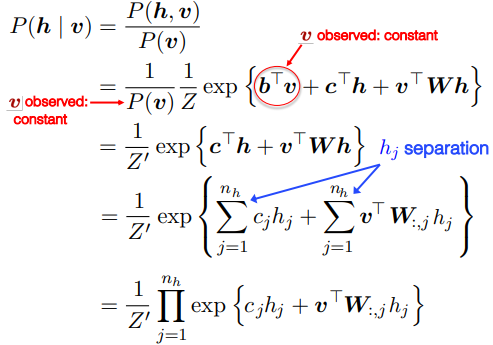
\includegraphics[]{images/pvh.png}
    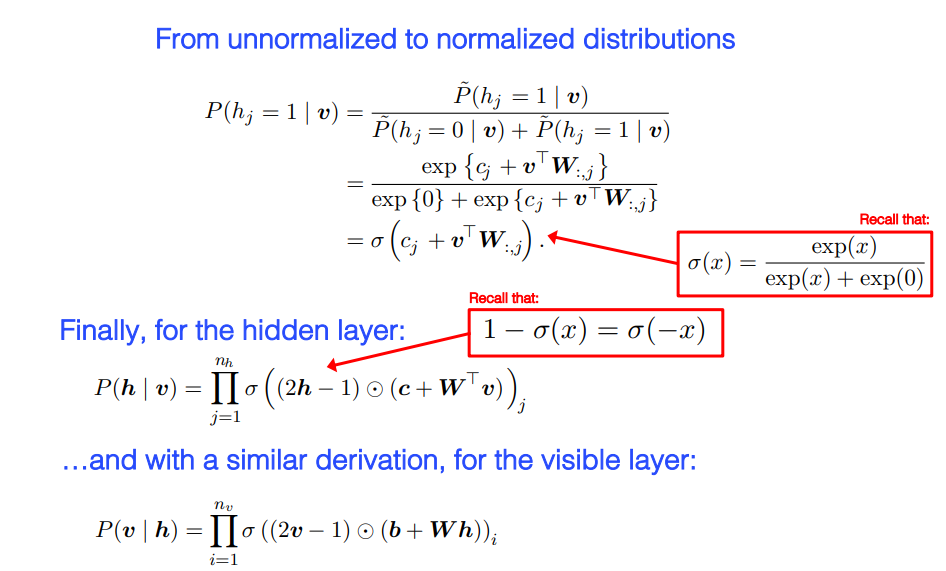
\includegraphics[scale=0.7]{images/pvh2.png}
\end{center}
Obviously, the latent variables' values are not observable from the data, but they are \textbf{inferred} by the model during training. Knowing $P(\textbf{h}|\textbf{v})$ and $P(\textbf{v}|\textbf{h})$ is useful to perform any kind of probabilistic task (e.g. $P(\textbf{v}|\textbf{h})$ can be used to generate new samples). The values of $\textbf{W}, \textbf{c}$ and $\textbf{b}$ need to be learned during training from data.
\newline\newline
Given training data $\textbf{x}$, we want to maximize the log-likelihood $log\,p(\textbf{x};\theta)$. However, its gradient with respect to $\theta$ is :
\[\nabla_\theta log\,P(\textbf{x};\theta) = \nabla_\theta log\,\Tilde{P}(\textbf{x};\theta) - \nabla_\theta log\, Z(\theta)\]
where $\Tilde{P}(\textbf{x};\theta)$ is the unormalized probability distribution defined by the RBM model, that is, $exp(-E(\textbf{v}, \textbf{h}))$. Computing this term is not a problem. However, the term $\nabla_\theta log\, Z(\theta)$ is usually intractable.\newline\newline
Under some conditions satisfied by RBMs (as well as most ML models), it can
be shown that:
\[\nabla_\theta log\, Z = E_{x \sim P(\textbf{x})}\nabla_\theta log\, \Tilde{P}(\textbf{x})\]
However, this is not possible to compute exactly since we need to sample $\textbf{x} \sim P(\textbf{x})$. Therefore, we must rely on some kind of approximation (Monte Carlo methods)\footnote{Note that approximating the gradients is not a big problem as we have seen with mini-batch algorithms}.\newline\newline
RBMs are usually trained using gradient ascent and Gibbs sampling to deal with the intractability of the partition function. The basic idea is that the weights are adjusted in order to minimize the difference between the reconstructed data and the original data.

\section{Monte Carlo Methods}
Randomized algorithms fall into two rough categories: Las Vegas algorithms and Monte Carlo algorithms. Las Vegas algorithms always return precisely the correct answer (or report that they failed). These algorithms consume a random amount of resources, usually memory or time. In contrast, \textbf{Monte Carlo} algorithms return answers with a random amount of error.

\subsection{Monte Carlo Sampling}
There are many reasons that we may wish to \textbf{draw samples} from a probability distribution. Sampling provides a flexible way to approximate many sums and integrals at reduced cost.\newline\newline
When a sum or an integral cannot be computed exactly, it is often possible to approximate it using Monte Carlo sampling. The idea is to view the sum or integral $s$ as if it was an expectation under some distribution $p$ and to approximate the expectation by a corresponding average. 
\begin{center}
    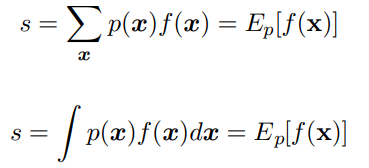
\includegraphics[scale=0.8]{images/Monte carlo.png}
\end{center}
We can approximate $s$ by drawing $n$ samples $\textbf{x}^{(1)}, ... \textbf{x}^{(n)}$ from $p$ and computing the empirical average:
\[\hat{s}_n = \frac{1}{n}\sum_{i=1}^n f(x^{i})\]
For very large $n$, the error converges “almost surely” to 0. However, sampling from $p(\textbf{x})$ is not always possible.

\subsection{Importance of sampling}
An important step in the decomposition of the sum or integral performed by Monte Carlo Sampling techniques is deciding which part of the integral (sum) should play the role of the probability $p(\textbf{x})$ and which part of the integral (sum) should play the role of the quantity $f(\textbf{x})$ whose expected value (under that probability distribution) is to be estimated. There is no unique decomposition because $p(\textbf{x})f(\textbf{x})$ can always be rewritten as:
\[p(\textbf{x})f(\textbf{x}) = q(\textbf{x})\frac{p(\textbf{x})f(\textbf{x})}{q(\textbf{x})}\]
where we now sample from $q$ and average from $\frac{pf}{q}$. Fortunately, we can easily compute the optimal importance sampling $q^*$ so to reduce variance:
\[q^*(\textbf{x}) = \frac{p(\textbf{x})|f(\textbf{x})|}{Z}\]
where $Z$ is the normalization constant, chosen so that $q^*$ sums or integrates to
1 as appropriate.

\subsection{Markov Chain}
In many cases, we wish to use a Monte Carlo technique but there is no tractable
method for drawing exact samples from the distribution $p(\textbf{x})$ or from a good (low variance) importance sampling distribution $q(\textbf{x})$. In the context of deep learning, this most often happens when $p(\textbf{x})$ is represented by an undirected model (such as RBM). In these cases, we introduce a mathematical tool called a Markov chain to approximately sample from $p(\textbf{x})$. The family of algorithms that use Markov chains to perform Monte Carlo estimates is called Markov chain Monte Carlo methods (MCMC).\newline\newline
The core idea of a Markov chain is to have a state $\textbf{x}$ that begins as an arbitrary value. Over time, we randomly update $\textbf{x}$ repeatedly. Eventually $\textbf{x}$ becomes (very nearly) a fair sample from $p(\textbf{x})$.\newline\newline
Formally, a Markov chain is defined by a random state $\textbf{x}$ and a transition distribution $T(\textbf{x}'| \textbf{x})$ specifying the probability that a random update will go to state $\textbf{x}'$ if it starts in state $\textbf{x}$. Running the Markov chain means repeatedly updating the state $\textbf{x}$ to a value $\textbf{x}'$ sampled from $T(\textbf{x}' | \textbf{x})$.\newline\newline
Let $q^{(t)}(x)$ the distribution at iteration $t$ from which $x$ is drawn. The goal is for $q^{(t)}(x)$ to converge to $p(x)$.\newline\newline
Let $i$ be an integer that represents a state. Then, we can describe $q(x)$ as a vector $\textbf{v}$ where $v_i = q(x=i)$. The probability of a single state landing in state $x'$ is given by:
\begin{equation}
    q^{(t+1)}(x') = \sum_x q^{(t)}(x)T(x'|x)
\end{equation}
We can represent the effect of the transition operator $T$ using a matrix $\textbf{A}$. We define $\textbf{A}$ so that:
\[A_{i,j} = T(x' = i | x=j)\]
$\textbf{A}$ is called a stochastic matrix, that is, (each of its columns represents a probability distribution.\newline\newline
Then, we can rewrite equation (1) in the following way:
\[\textbf{v}^{(t)} = \textbf{A}\textbf{v}^{(t-1)}\]
It can be shown that the process of applying the Markov Chain update repeatedly eventually converges to a \textbf{stationary distribution}, sometimes also called the \textbf{equilibrium distribution}:
\[\textbf{v}' = \textbf{Av} = \textbf{v}\]
If we have chosen $T$ correctly, then the stationary distribution $q$ will be equal to the distribution $p$ we wish to sample from.

\section{Gibbs sampling}
In the context of deep learning, we commonly use Markov chains to draw
samples from an energy-based model defining a distribution $p(\textbf{x})$. In this case, we want the $q(\textbf{x})$ for the Markov chain to be $p(x)$. To obtain the desired $q(\textbf{x})$, we must choose an appropriate $T(x' | x)$.\newline\newline
A conceptually simple and effective approach for building a Markov chain
that samples from $p(\textbf{x})$ is to use \textbf{Gibbs sampling}, in which sampling from $T(\textbf{x}' | \textbf{x})$ is performed by selecting one variable $x_i$ and sampling it from $p$ conditioned on its neighbors in the undirected graph $G$ defining the structure of the energy-based model.\newline\newline
It is also possible to sample several variables at the same time so long as they are conditionally independent given all of their neighbors. All of the hidden units of an RBM may be sampled simultaneously because they are conditionally independent from each other given all of the visible units. The same is valid also for the visible variables. Gibbs sampling approaches that update many variables simultaneously in this way are called \textbf{block Gibbs sampling}.\newline\newline
Usually in deep learning we just run the process for $n$ steps, for some $n$ that we think will be big enough, and hope for the best.
